\section{Let's the fun begin!}
\newthought{We are left to define derivatives} of functions between manifolds.
And, since we saw that euclidean spaces are manifolds, we better find a definition that coincides with the one you saw in your analysis courses.

\begin{marginfigure}[7em]
  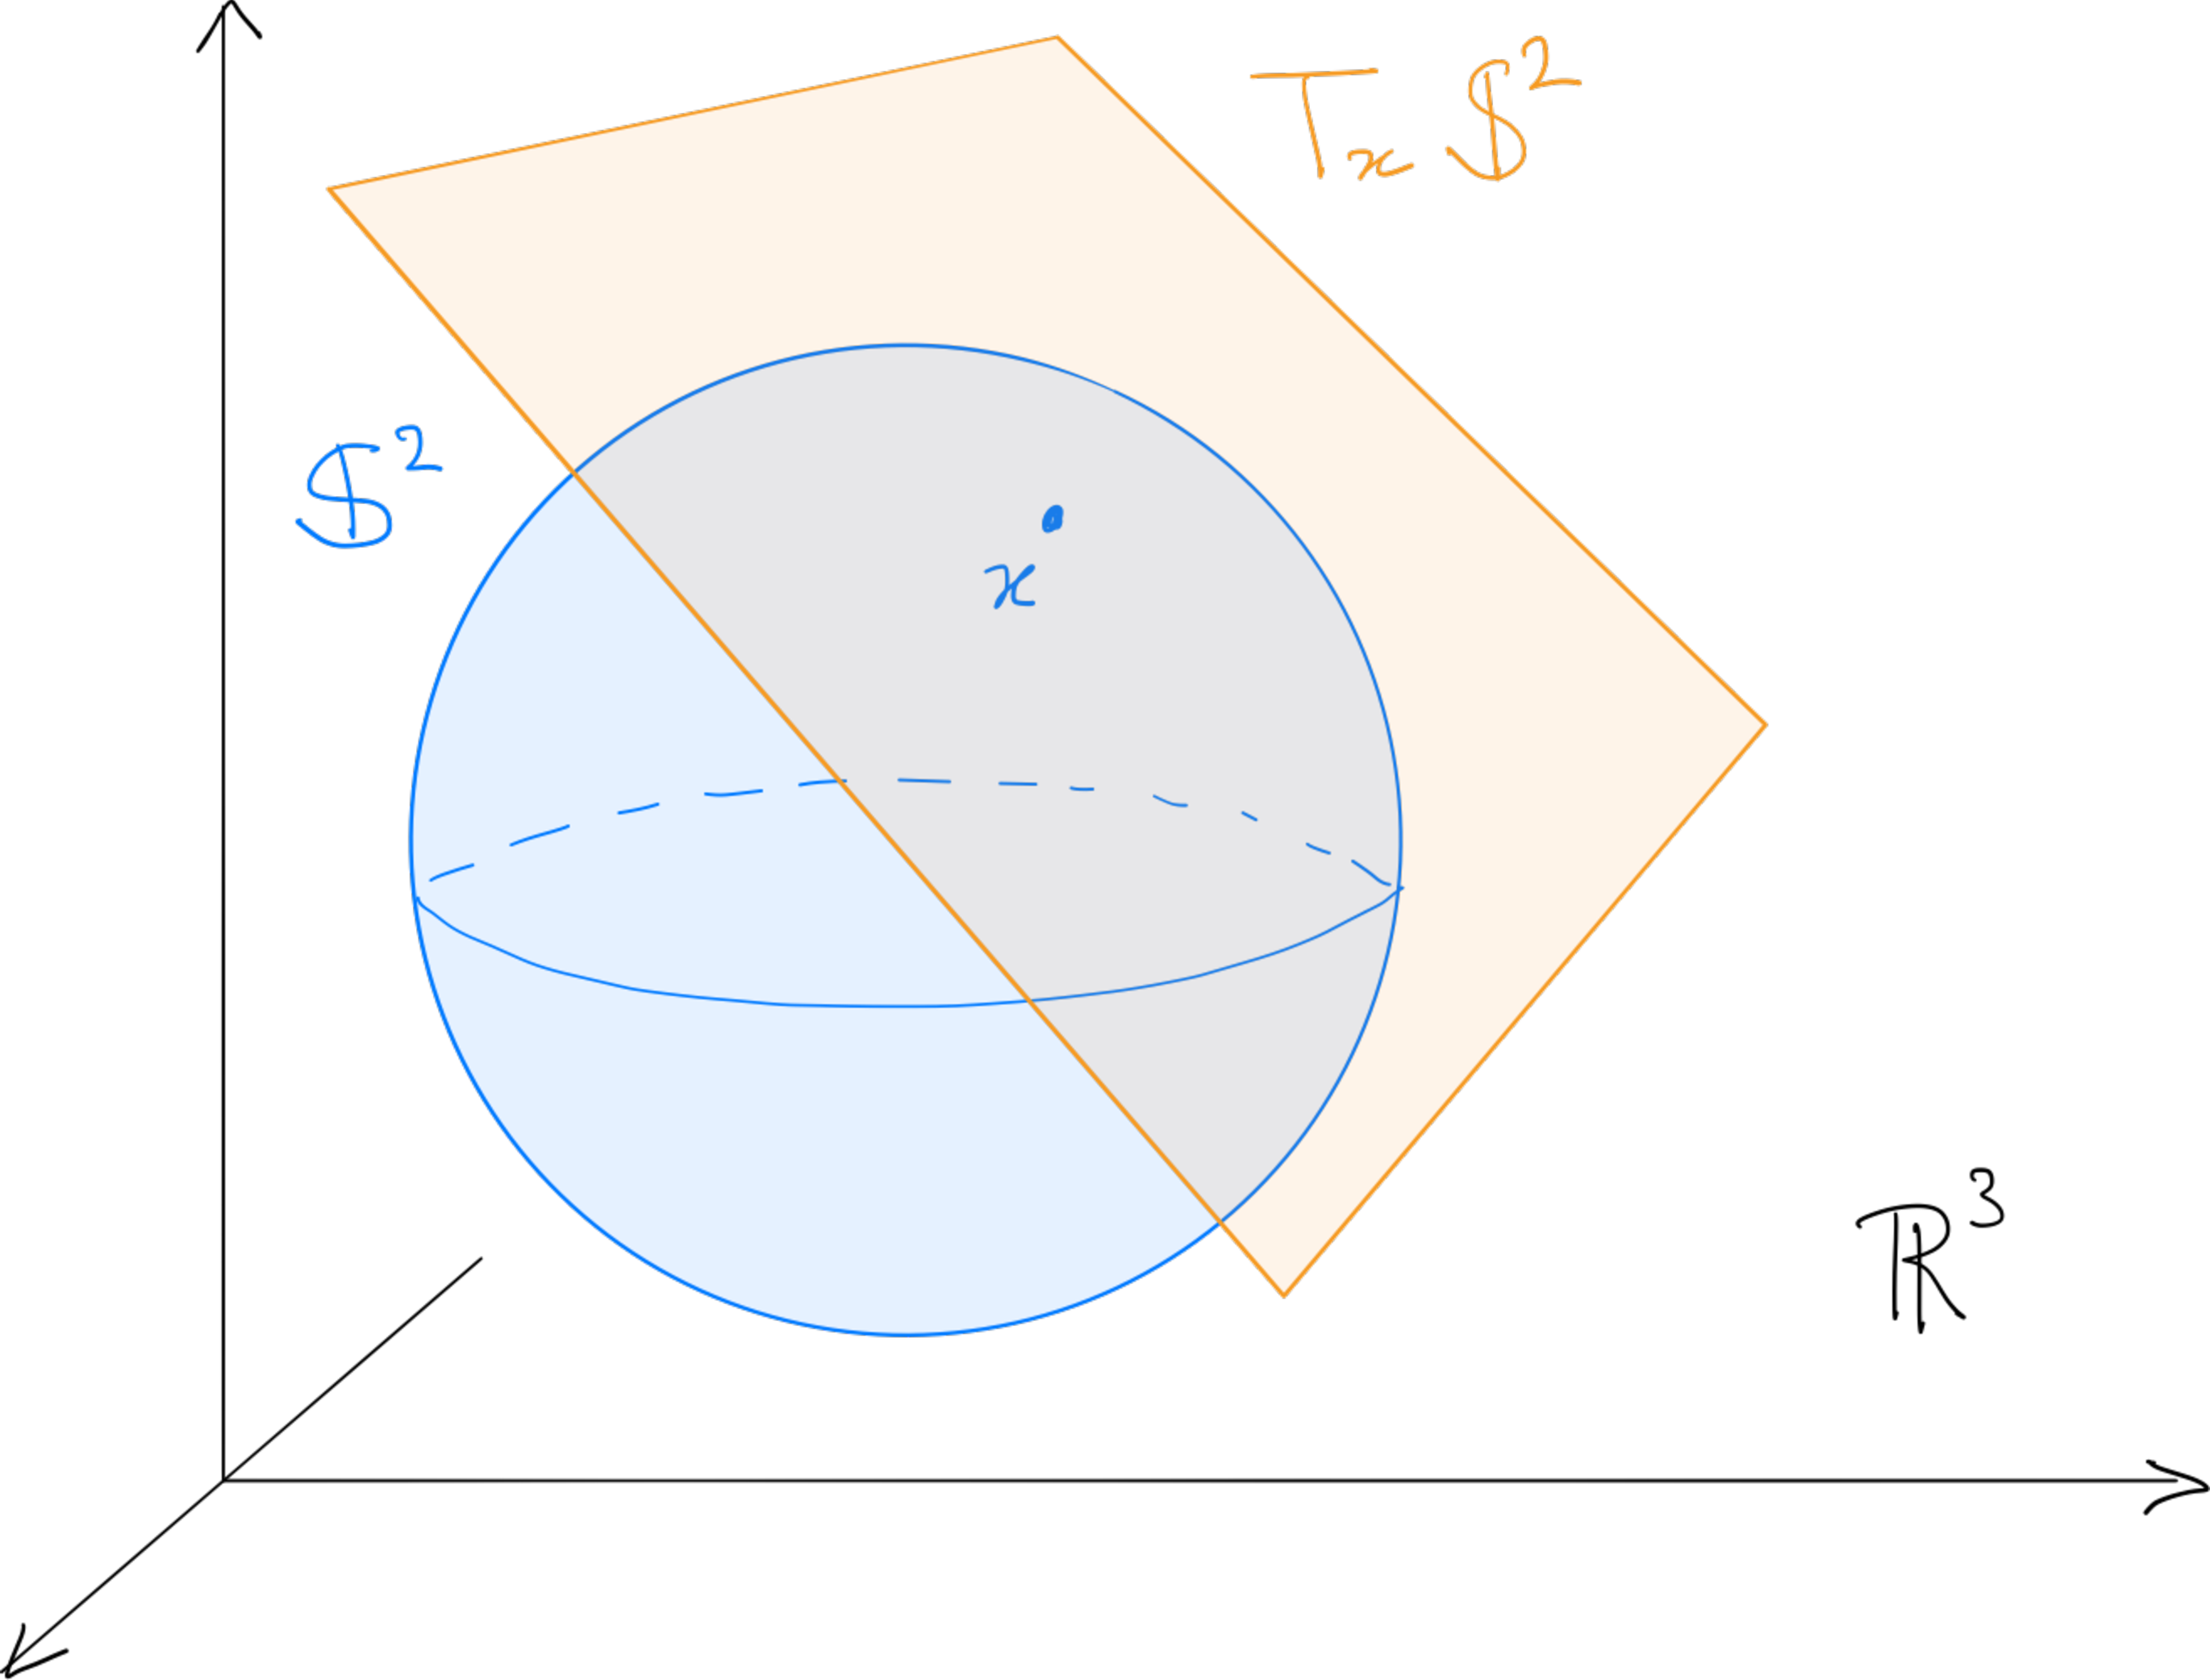
\includegraphics{2_1-embedded-sphere-tangent.pdf}
  \label{fig:tan-embedded-sphere}
  \caption{Tangent space to a point of a sphere $\bS^2$ embedded into the ambient space $\R^3$.}
\end{marginfigure}
In this chapter we will see how to associate to an $n$-dimensional smooth manifold $M$ an $n$-dimensional vector space, denoted by $T_x M$, to each point $x\in M$.
Such vector space is called \emph{tangent space to $M$ at $x$} and, for a manifold embedded into a euclidean ambient space, it will coincide with the intuitive understanding of a tangent hyperplane to the point on the manifold, see also Figure~\ref{fig:tan-embedded-sphere}.
As we will see, there are various different definition of tangent space but, in the end, they all turn out to be equivalent.

Due to the amount of freedom and the many equivalent definitions, there is no unique way of introducing tangent spaces.
Just to give you an idea, all the following approaches lead to equivalent definitions (see also \cite{book:lee}):
\begin{enumerate}
  \item equivalence classes of curves through a point;
  \item transformation laws of the components of vectors with respect to different charts;
  \item generalization of linear approximation into the idea of an abstract derivation;
  \item derivations in the category of germs of functions;
\end{enumerate}

It is also possible to ``flip'' the whole construction around, constructing differentials and cotangent spaces and using them to introduce the tangent spaces.
This is the approach taken by \cite{lectures:hitchin} and it is at least worth of a look if you want to see a different perspective.

To avoid diverging from the book too much, we will stick to derivations on the space of germs, which emphasizes the locality of derivations to an extreme.
The equivalence between our approach and the one based on speeds of curves and on derivations will be left as homeworks.

\section{Directional derivatives in euclidean spaces}

Suppose that $f: U\subset\R^n\to\R^k$ is a smooth map defined on an open subset $U\subset \R^n$.
In multivariable calculus you have seen that if $x\in U$ and $v\in\R^n$, then the vector $Df(x) v$ can be interpreted as the directional derivative\footnote{Sometimes this is denoted $D_v f(x)$ instead.} of $f$:
\begin{equation}
    Df(x) v = \lim_{t\to0}\frac{f(x+tv) - f(x)}{t}.
\end{equation}
Then, the partial derivative is obtained as the particular case
\begin{equation}
    D_jf(x) := Df(x) e_j = \lim_{t\to0} \frac{f(x+te_j) - f(x)}{t}.
\end{equation}
Of course, we can also look at the derivative by using the standard euclidean coordinates $r^1, \ldots, r^n$, in that case we would be deriving $r^i \circ f : \R^n \to \R$.

\newthought{Let's take it slow}, and compare all these various derivatives next to each other.
For $f:U\subset\R^n\to\R^k$ and $x\in U$, we have
\begin{marginfigure}[3.5cm]
    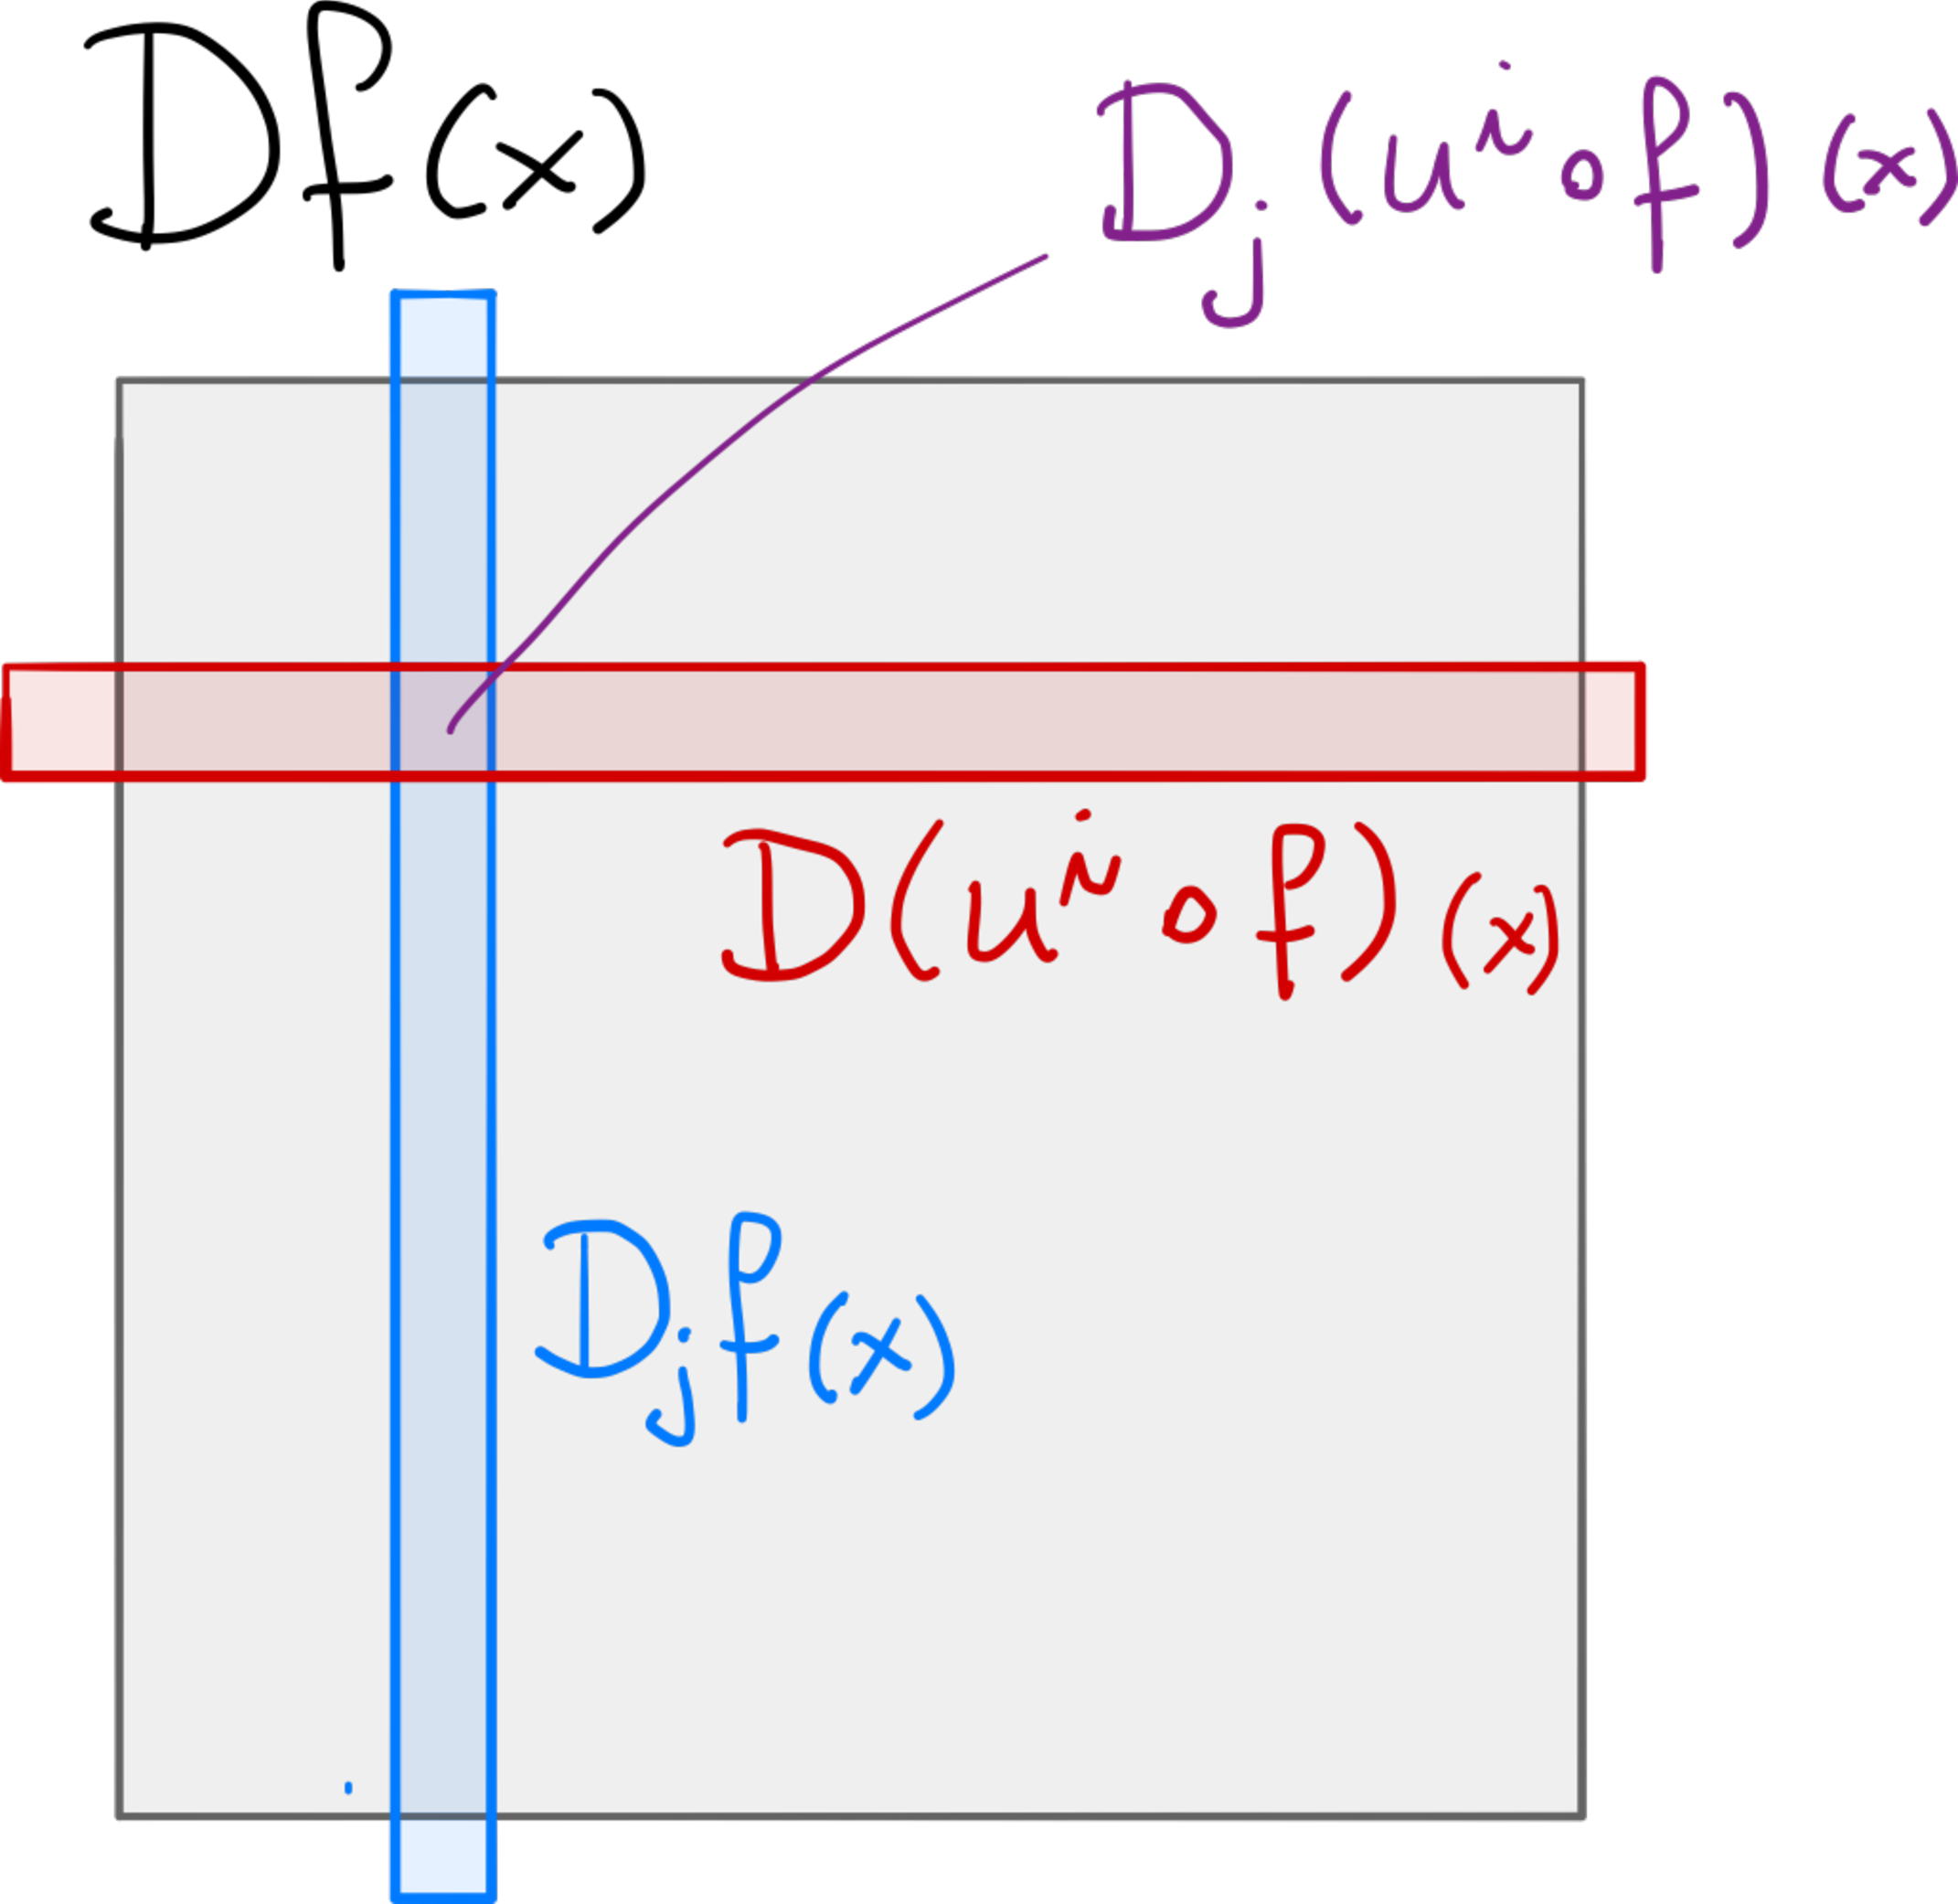
\includegraphics{2_3-ederivs.pdf}
\end{marginfigure}
\begin{itemize}
    \item $Df(x)$, the Jacobian matrix, which is a $k\times n$ matrix;
    \item $D_j f(x)$, the $j$th column of the matrix $Df(x)$, which is an element of $\R^k$;
    \item $D(r^i\circ f)(x)$, a linear function from $\R^n to \R$, which one can think as the $i$th row of the matrix $Df(x)$;
    \item $D_j(r^i\circ f)(x) = \frac{\partial f^i}{\partial x^j}(x)$, a number in $\R$, which corresponds to the element $(i,j)$ of the matrix $Df(x)$.
\end{itemize}

This notation using $D$ instead of spelling out the partial derivatives, comes with an important advantage.
Let's use it to rewrite the chain rule form Proposition~\ref{thm:chainrule}(\ref{thm:chainrule2}):
\begin{equation}
    D_j(u^i\circ g \circ f) (x) = \sum_{r=1}^k D_r(u^i\circ g)(f(x))\; D_j(u^r \circ f)(x),
\end{equation}
where $1\leq i\leq m, 1\leq j \leq n$.
As you cen see, we did not need to spell out explicitly the coordinate systems on $\R^n$ or $\R^k$.

\section{Germs and derivations}

\newthought{To reach our goal of defining derivations on manifolds}, a direct extension of partial derivatives is not enough: we will need to introduce some more levels of abstraction.

\begin{defn}
    Let $M$ be a smooth manifold.
    For some point $p\in M$, let $U,V\subset M$ be two neighborhoods of $p$.
    We say that two functions $f\in C^\infty(U)$ and $g\in C^\infty(V)$ have the same \emph{germ} at $p$ if there exists a neighborhood $W\subset U\cap V$ of $p$ such that $f|_W \equiv g|_W$.
\end{defn}

Germs define an equivalence relation on the set of smooth functions defined on a neighborhood of a point $p$: $(U, f) \sim_p (V, g)$ if they have the same germ at $p$. Then, a germ $[f]_p$, where $(U, f)$ is one representative for $[f]_p$, is an equivalence class in the quotient space 
\begin{equation}
    C_p^\infty(M) := C^\infty(M)/\sim_p.
\end{equation} 

\begin{exe}
    Show that $\sim_p$ defined above is an equivalence relation in $C^\infty(M)$.
\end{exe}

For $c\in\R$ and $[f]_p, [g]_p$ germs with representatives $(U, f), (V, g)$, we have
\begin{itemize}
    \item $[f]_p + [g]_p$ is the germ with representative $(U\cap V, f+g)$;
    \item $[f]_p [g]_p$ is the germ with representative $(U\cap V, f g)$;
    \item $c[f]_p$ is the germ with representative $(U, cf)$.
\end{itemize}
Therefore, $C_p^\infty(M)$ is also an algebra over $\R$.

Germs are the apotheosis of locality: a germ at $p$ has a well defined value at $p$ and nowhere else.
This results in a map,
\begin{equation}
    \eval_p: C_p^\infty(M) \to \R, \quad
    \eval_p([f]_p) := f(p),
\end{equation}
where $(V,f)$ is any representative of $[f]_p$.

We can now go back to our discussion of euclidean derivations to motivate our definition of tangent vectors.

\begin{ex}\label{ex:euclideanD}
    Let $U\subset\R^n$ open\footnote{In what follows, we will think at $U$ both as an open subset of $\R^n$ and a smooth manifold depending on what is most convenient for us.} and $f\in C^\infty(U)$.
    For $x\in U$ and $v\in\R^n$ we have seen that $Df(x)$ can be interpreted as a matrix that consumes the vector $v$ to produce a number $D(f)v$.
    In such interpretation $f$ is fixed and only $x$ and $v$ vary, however there is no reason for this restriction.

    Indeed, an alternative interpretation lets also $f$ vary and consider the action of differentiation as a map
    \begin{equation}
        U \times \R^n \times C^\infty(U) \to \R,\quad
        (x,v,f) \mapsto Df(x) v.
    \end{equation}
    And since we are flipping around all the ideas, let us consider $x$ and $v$ fixed and instead only let $f$ vary:
    \begin{equation}\label{eq:mapxvtoD}
        (x,v):C^\infty(U) \to\R, \quad (x,v)(f) := Df(x)v.
    \end{equation}.
    By the definition \eqref{eq:diff} of the euclidean differential, we know that it is a local property: the value $Df(x)$ only depends on the germ of $f$ at $x$.
    Thus we can rephrase \eqref{eq:mapxvtoD} by saying that $v$ defines a \emph{linear} map
    \begin{equation}
        v : C_p^\infty(U) \to \R, \quad
        v([f]_p) := Df(x) v.
    \end{equation}
    In fact, this is not just a linear map, it also satisfies a \emph{derivation} property, in the sense that
    \begin{equation}
        v([f]_p [g]_p) =
            \eval_p([f]_p)v([g]_p)
            + \eval_p([g]_p)v([f]_p).
    \end{equation}
    Which, rewritten in a more familiar form, is just a way to rewrite the \emph{Leibniz rule}:
    \begin{equation}
        D(fg)(x) v = f(x)Dg(x)v + g(x) Df(x)v.
    \end{equation}

    Note that we have now two different interpretations for $v$: it is both a vector in $\R^n$ and a linear map $C_p^\infty(U) \to \R$ satisfying the derivation property.
\end{ex}

Motivated by Example~\ref{ex:euclideanD}, we will define a tangent vector as a derivation on the space of germs.

\begin{defn}
    Let $M$ a smooth manifold of dimension $n$ and let $p\in M$.
    A \emph{tangent vector at $p$} is a linear map
    \begin{equation}
        v: C_p^\infty(M)\to\R
    \end{equation}
    which is also a derivation, i.e.
    \begin{equation}
        v([f]_p [g]_p) =
            \eval_p([f]_p)v([g]_p)
            + \eval_p([g]_p)v([f]_p).
    \end{equation}

    Since a tangent vector is a linear map from the vector space $C_p^\infty(M)$ to $\R$, the set of all tangent vectors at a point $p$ is itself a vector space\footnote{Exercise: why is this true?} which we denote by $T_p M$.
\end{defn}

Let's check that these vectors, at least satisfy the most elementary properties of derivations: one would expect the derivative of constant functions to be zero, is that the case?

\begin{lem}
    Let $M$ be a smooth manifold, let $U\subset M$ be an open set containing $p$ and let $v\in T_p M$.
    Denote by $[c]_p$ the germ of a constant function $(U, p \mapsto c)$.
    Then $v([c]_p) = 0$.
\end{lem}
\begin{proof}
    Since $[c]_p = c [1]_p$, by linearity we have $v([c]_p) = c v([1]_p)$.
    Thus, it will be enough to show that $v([1]_p) = 0$.
    Since $v$ is a derivation, using the algebra properties of the space of germs we get
    \marginnote{Keep this simple trick in mind, it will be useful in the future.}
    \begin{equation}
        v([1]_p) = v([1]_p [1]_p) = 2 \eval_p([1]_p)v([1]_p) = 2 v([1]_p).
    \end{equation}
    Thus, $v([1]_p) = 0$, concluding the proof.
\end{proof}

As you can see, working with equivalent classes is doable but unnecessarily cumbersome. As we did with atlases, we would like to get it over with.

\begin{defn}
    Let $M$ be a smooth manifold and $p\in M$.
    Let $W\subseteq M$ be any neighborhoods of $p$.
    A \emph{derivation of $C^\infty(W)$ at $x$} is a linear map $w:C^\infty(W)\to\R$ which satisfies Leibniz rule
    \begin{equation}
        w(fg) = f(p)w(g) + g(p)w(f).
    \end{equation}
\end{defn}

If $v\in T_p M$, then we already saw that $v$ naturally defines a derivation $w$ of $C^\infty(W)$ for any open neighborhood $W$ of $p$. In this case $w(f) := v([f]_p)$.

\textcolor{red}{\hrulefill}

A map $\gamma\in\cC^1(I, M)$ from an open interval $I\subset\R$ to a smooth manifold $M$ is called \emph{$\cC^1$-curve} on $M$.
\begin{marginfigure}
  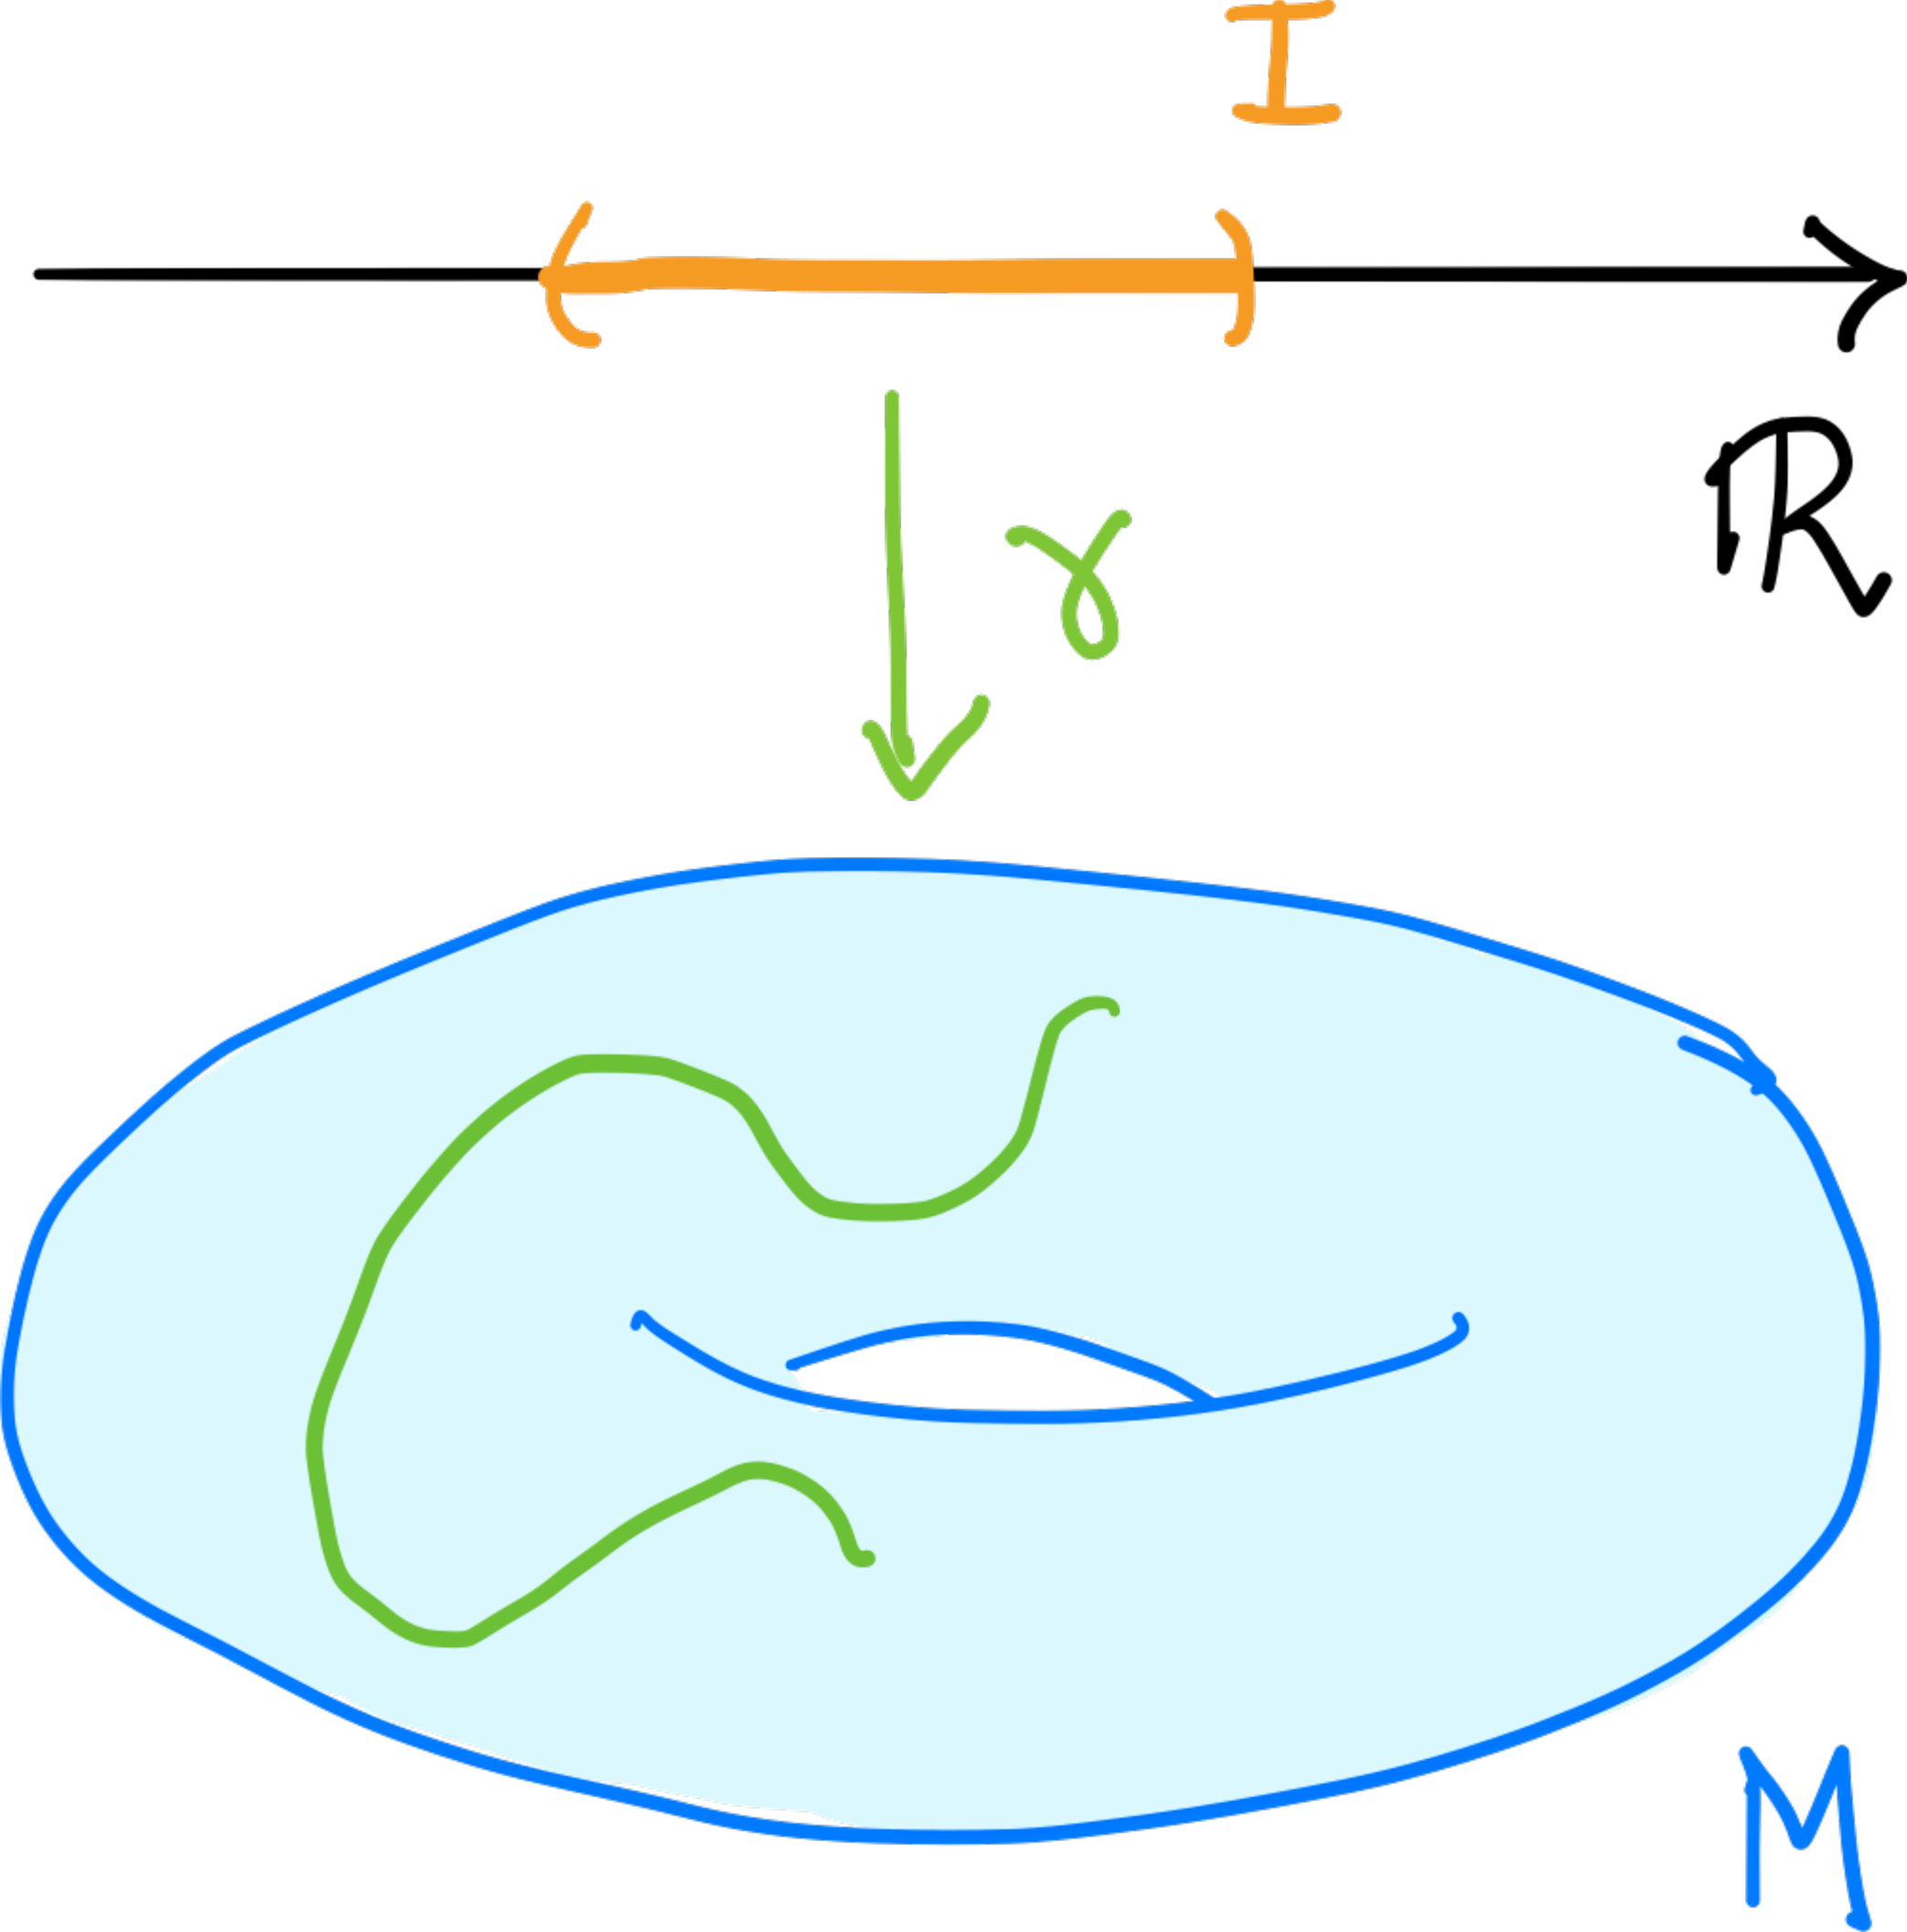
\includegraphics{2_2-curve-on-M.pdf}
\end{marginfigure}
F
\section{Via charts}
\section{As derivation}

\section{A summary}

\section{The tangent bundle}